% !TEX encoding = UTF-8
% !TEX TS-program = pdflatex
% !TEX root = ../main.tex
% !TEX spellcheck = en-GB

\documentclass[final, 11pt, a4paper, titlepage]{article}
\makeatletter
\AtBeginDocument{\let\hl\@firstofone}
\makeatother

\usepackage[english]{babel}
\usepackage[utf8]{inputenc}
\usepackage[hidelinks]{hyperref}
\usepackage{graphicx}
\usepackage{textcomp}
\usepackage{wallpaper}
\usepackage{color}
\usepackage{mathtools}
\usepackage{listings}
\usepackage{amssymb}
\usepackage[
	backend=biber,
	citestyle=numeric-comp,
	hyperref,
	backref,
	sorting=none
]{biblatex}

\graphicspath{{images/}}

\addbibresource{bibliography.bib}


\defbibheading{bibliography}
{
    \phantomsection 
    \addcontentsline{toc}{section}{\bibname}
    \section*{\bibname\markboth{\bibname}{\bibname}}
}

\setlength\bibitemsep{1.5\itemsep} 

%\DeclareBibliographyCategory{sampleCategory}

%\addtocategory{sampleCategory}{referenceID}


\newcommand{\university}{Università degli Studi di Padova}
\newcommand{\dept}{Department of Mathematics}
\newcommand{\faculty}{Master Degree in Computer Science}
\newcommand{\myyear}{Academic Year 2016/17}
\renewcommand{\title}{QuizFight}
\newcommand{\subtitle}{An Android trivia quiz application}
\newcommand{\fstauthor}{Alex Beccaro - 1156235}
\newcommand{\sndauthor}{Emanuele Carraro - 1155105}
\newcommand{\trdauthor}{Matteo Di Pirro - 1154231}

\begin{document}
	\begin{titlepage}
\begin{center}

\begin{LARGE}
\textbf{\university}\\
\end{LARGE}

\vspace{10pt}

\begin{Large}
\textsc{\dept}\\
\end{Large}

\vspace{10pt}

\begin{large}
\textsc{\faculty}\\
\end{large}

\vspace{30pt}
\begin{figure}[htbp]
\begin{center}

\includegraphics[height=6cm]{images/logo_unipd}
\end{center}
\end{figure}
\vspace{30pt} 

\begin{LARGE}
\begin{center}
\textbf{\title}\\
\end{center}
\end{LARGE}

\begin{Large}
	\begin{center}
		\textbf{\subtitle}\\
	\end{center}
\end{Large}

\vspace{20pt} 

\begin{large}
\begin{flushright}
\textit{\fstauthor \\ \sndauthor \\ \trdauthor}
\end{flushright}
\end{large}

\vspace{40pt}

\line(1, 0){338} \\
\begin{normalsize}
\textsc{\myyear}
\end{normalsize}

\end{center}
\end{titlepage} 
	\tableofcontents
	\newpage
	\section{Introduction}

The benefits of a gaming approach for learning are well-known. In fact,
people learn better and more when they play games. We are never tired of
playing.
After all, games mean fun. And fun means that our minds are relaxed and open
for gaining new knowledge.
This is why, over the last few years, scientists have begun to commission
more and more scientific games.
The goal is to involve people in science and let them learn new things.

Furthermore, nowadays there are many game shows that let people test their
trivia knowledge.
They are fun and useful because they allow both competitors and audience to
learn new things, while playing.
We develop QuizFight, a trivia quiz application allowing users to test their
trivia knowledge.
Contrariwise to popular game shows, we cannot reward users with money.
Instead they gain experience. 

The basic flow is simple. We identify a set of 20 topics and users can
dare each other with duels in three different topics.
Users can also choose to generate random topics for a duel.
Hence, a duel comprises of three different rounds each of which comprises
of five questions.
Each question has an associate difficulty level determining its score.
Difficulty levels range in [1, 3].
There are almost 1000 different questions available.

QuizFight ``programmatic'' goal is, on the other hand, to test how easily an
Android application can interact with different well-known service providers,
such as Google Play Services and Facebook.

We found that using their services is pretty simple, even if the learning curve
is not so linear.

In this paper we explain some QuizFight features and how they are
implemented.
We also discuss some current limitations and provide likely directions for
future work. 

The rest of this paper is organized as follows. Section~\ref{ref:design} explains
some design details. Section~\ref{sec:server} describes the choices we made for
QuizFight's server and how the Android application interacts with it. 
Section~\ref{sec:fcm} is about how notifications are sent to the clients.
Sections~\ref{sec:fb} and \ref{sec:ggames} illustrate how our application
interacts with both Facebook and Google for providing a consistent user
experience. Sections~\ref{sec:issues} describes some known issues due 
our use of Google Games. Our work is then concluded in Section~\ref{sec:limitations},
where we provide some lines for further work.
	
	\section{Application design}\label{ref:design}

QuizFight information model is depicted in Figure \ref{fig:quizfighter}.
The main entry point is \texttt{SignInActivity}.
Our game, in its very first version, requires the user to sign in with Google
Games. Hence, \texttt{SignInActivity} simply shows a button for the sign in.
The user's dashboard is \texttt{HomeActivity}.
Here the player can see their previous duels, both the completed and the
pending ones.
By tapping on a duel, a complete report of the result is shown.
When the duel has not been completed and when a new round is actually
available (i.e. when both the player and their opponent completed the
previous round), a button asking the user for answering the next questions
is shown.
Since showing every duel would incur in a bad user experience we show
only a limited number. We then provide a way to see the complete lists.

\begin{figure}[t]
	\centering
	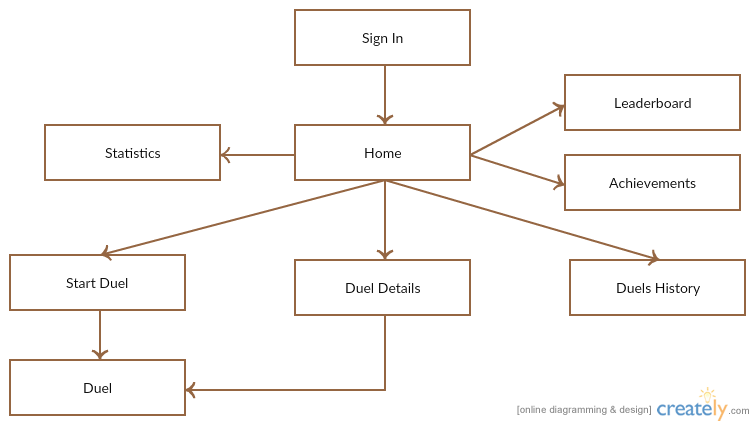
\includegraphics[width=0.9\linewidth]{QuizFightER}
	\caption{QuizFight information model}
	\label{fig:quizfighter}
\end{figure}

From \texttt{HomeActivity} a user can also see their current situation in terms
of ranks and achievements.
That information is directly retrieved and shown using Google's services.
In addition, QuizFight offers the possibility to take a look at a user's
statistics, such as the number of duels (or rounds) won versus the number of
duels (or rounds) played and the correct answers.
All these statistics are presented in bar charts.
Finally, there is the possibility to sign in with Facebook, for daring the
user's friends.

By tapping on the fight button it is possible to start a new duel.
Here, the adversary can be chosen in three different modalities:

\begin{itemize}
	\item \textbf{random};
	\item selected from the \textbf{leaderboard};
	\item selected from the \textbf{Facebook's friends list}.
\end{itemize}

After \texttt{DuelActivity} is shown, the user is able to answer the
questions of the round. At the round's ending a dialog is shown to notify 
the user about their actual round's score. If both the player and the opponent 
have terminated the current round they are both notified about a new round 
available (if any), or about the duel's ending (with the final score). 

	
	%%bibliography
	%\newpage
	%\nocite{*}
	%\printbibliography 
	
\end{document}